\section{Principali punti di estensione}
\NomeProgetto{} è una web app progettata pensando anche ad eventuali operazioni future di manutenzione o estensione del prodotto. Rispetto alla manutenzione del codice essa è favorita da una codifica coerente in tutti i file (grazie all'utilizzo di ESLint per l'analisi statica) e l'aggiunta di commenti ove necessario.
Riguardo l'estensibilità dell'applicazione sono stati individuati principalmente tre funzionalità che potranno essere ampliate senza grandi difficoltà.

\subsection{Riduzione dimensionale}
Come detto in precedenza questa funzionalità è stata implementata con l'utilizzo dello strategy pattern. Questo permette una facile manutenzione delle classi concrete degli algoritmi già presenti e permette l'estensione con altri algoritmi di riduzione dimensionale, senza la necessità che essi siano presenti nella libreria Druid.js (attualmente utilizzata a questo scopo). L'implementazione del metodo \texttt{startDR()} in un nuovo algoritmo è infatti indipendente dalle altre già preesistenti. È necessario però aggiungere anche una classe per contenere i corrispondenti parametri, la quale estende la classe astratta \textit{Parameter} (fare riferimento al diagramma dello strategy pattern alla sezione \S 6.4).

\subsection{Calcolo della distanza}
Il calcolo della distanza risulta facilmente estendibile con nuove funzioni. È infatti sufficiente seguire i seguenti passi: 
\begin{enumerate}[label=\textbf{\arabic*})]
	\item Aggiungere i nuovi tipi di distanza nell'oggetto \texttt{DistanceType} (riportato in figura \ref{distancetype}) presente nel file \textbf{utils.js};
	\item Aggiungere le corrispondenti \texttt{option} all'interno della form di selezione (riportata in figura \ref{distanceoption}). Essa si trova nel file \textbf{DistanceCalculation.js} all'interno del \texttt{return()} del componente React.
\end{enumerate}

L'unico vincolo è che, per non dover cambiare nient'altro nel codice, le nuovi funzioni da aggiungere siano presenti all'interno della libreria \textit{ml-distance}, utilizzata a tale scopo. Essa ne fornisce molte, identificabili nella documentazione ufficiale:  
\begin{center}
	\textcolor{blue}{\url{https://www.npmjs.com/package/ml-distance}}
\end{center}


\begin{figure}[!htb]
\minipage{0.32\textwidth}
	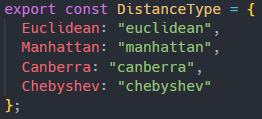
\includegraphics[width=\linewidth]{Images/oggdistance}
	\caption{Oggetto contenente i diversi tipi di distanza}
	\label{distancetype}
\endminipage\hfill
\minipage{0.65\textwidth}
	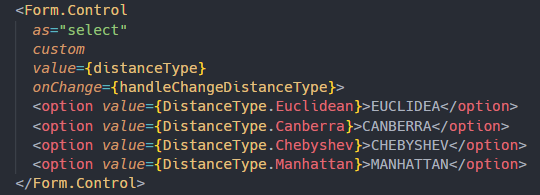
\includegraphics[width=\linewidth]{Images/calcdistance}
	\caption{Codice per l'input della funzione di calcolo della distanza}
	\label{distanceoption}
\endminipage
\end{figure}

\newpage 
\subsection{Visualizzazione dei dati}
\NomeProgetto{} fornisce cinque diversi tipi di visualizzazione dei dati caricati. È possibile aggiungerne di nuovi seguendo i seguenti passi:
\begin{enumerate}[label=\textbf{\arabic*})]
	\item Aggiungere i nuovi tipi di visualizzazione nell'oggetto \texttt{VisualizationType} (riportato in figura \ref{vistype}) presente nel file \textbf{utils.js};
	\item Aggiungere nel menu la corrispettiva voce per avviare la visualizzazione. In particolare bisogna aggiungere dei "case" nello switch dedicato (riportato in figura \ref{switchmenu}) che si trova in \textbf{MenuVM.js};
	\item A questo punto bisogna creare i file per le preferenze e per il grafico stesso. In particolare è necessario aggiungere i file:
	\begin{itemize}
		\item \textbf{NuovaVisualizzazionePreferences.js} e il corrispettivo \textit{ViewModel} nella cartella al percorso:
	\begin{center}
		\texttt{./src/components/UI/graphUI/preferences} ;
	\end{center}			
		
		\item \textbf{NuovaVisualizzazione.js} e il corrispettivo \textit{ViewModel} nella cartella al percorso:
	\begin{center}
		\texttt{./src/components/UI/graphUI/charts} .
	\end{center}		
	\end{itemize}		
	\item Per mostrare a schermo le nuove preferenze e i nuovi grafici è infine necessario aggiungere i "case" agli switch dedicati alla loro renderizzazione (riportati nelle figure \ref{switchpref} e \ref{switchchart}) nel file \textbf{Chart.js}.
\end{enumerate}

\begin{figure}[!htb]
\minipage{0.42\textwidth}
	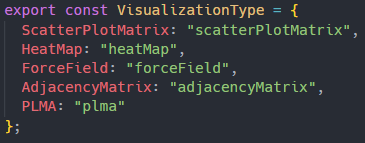
\includegraphics[width=\linewidth]{Images/vistype}
	\caption{Oggetto contenente i diversi tipi di visualizzazione}
	\label{vistype}
\endminipage\hfill
\minipage{0.55\textwidth}
	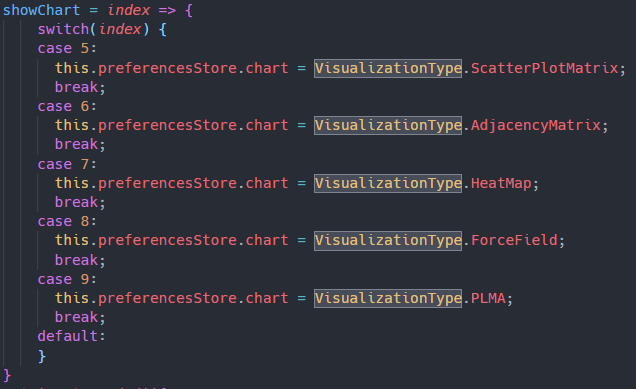
\includegraphics[width=\linewidth]{Images/menu}
	\caption{Switch per le voci del menu dedicate ai grafici}
	\label{switchmenu}
\endminipage
\end{figure}

\afterpage{
\begin{figure}[H]
\minipage{0.49\textwidth}
	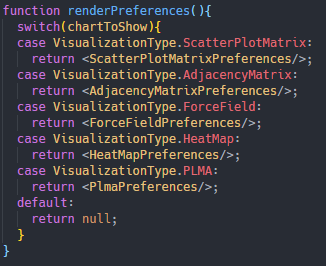
\includegraphics[width=\linewidth]{Images/renderpref}
	\caption{Switch per il rendering delle preferenze}
	\label{switchpref}
\endminipage\hfill
\minipage{0.48\textwidth}
	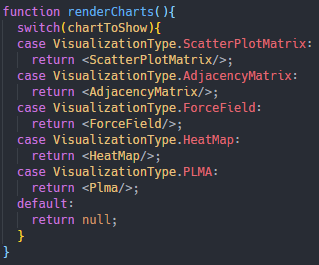
\includegraphics[width=\linewidth]{Images/renderchart}
	\caption{Switch per il rendering del grafico}
	\label{switchchart}
\endminipage
\end{figure}
\clearpage
}
